% Physics for Friends
% by Age

%- Preamble - Age - Article --


\documentclass{article}

%-------- Include Packages -----------
\usepackage{graphics}
\usepackage{wrapfig}
\usepackage{xcolor} % For colouring hyperlinks
\usepackage{tikz}
\usepackage[colorlinks=true,linkcolor={red!80!black},citecolor={blue!50!black},urlcolor={blue!80!black}]{hyperref}
\usepackage{tikz-3dplot}
% -- Math Related -------------------
\usepackage{amsmath}
\usepackage{mathtools}
\usepackage{latexsym}
\usepackage{mathrsfs} 	% Curly Math text for Lagrangians
\usepackage{esvect} 	% Allows vector arrow superscripts	
%----------- Particle Physics --------
\usepackage{feynmp-auto}
% ---------------- -------------------
%------- Custom Environments --------
\newcommand{\abs}[1]{\lvert#1\rvert}
\newcommand{\secref}[1]{[\ref{#1}]}
\newcommand{\sgn}{\operatorname{sgn}}
\newcommand{\abox}[1]{\vspace{0.3cm} \fbox{\addtolength{\linewidth}{-2\fboxsep} \addtolength{\linewidth}{-2\fboxrule} \begin{minipage}{\linewidth}#1 \end{minipage}}\vspace{0.3cm}}
\DeclarePairedDelimiter{\ceil}{\lceil}{\rceil}
\DeclarePairedDelimiter{\floor}{\lfloor}{\rfloor}
%------------------------------------

%----------Custom Variables ---------
% Define File Paths
\graphicspath{{Imgs/}}
\def \RefPath {../../References/}
\def \ImagePath {./Images/}
%------------------------------------
%-------- Page Typesetting -----------
\textwidth 17 truecm 
\textheight 23.5 truecm 
\topmargin -2 truecm 
\oddsidemargin -.2 truecm 


%------------Formatting --------------
% Remove Indenting
%\setlength{\parindent}{0cm}
% Change height of tables
\renewcommand{\arraystretch}{1.2}

%--------- Custom Settings -----------
%-------------------------------------

%--------- Title/Author --------------


%\title{}

%-------------------------------------



%\begin{document}




%\bibliographystyle{plain}
% \bibliography{../../../References/General, ../../../References/SUSY} %For vim-latex auto-completion
%\bibliography{\RefPath General \RefPath SUSY}

%\end{document}


\begin{document}
\section*{Physics for Friends}

~

\subsection*{Introduction}

I have written these incredibly brief (and hopefully pedagogical) notes with the intent of explaining some of the main concepts of modern theoretical physics to an audience with a high school or first year level background in maths and physics. I'll aim to do this over a handful of lectures, in a colloquial form designed casually for friends and family over a few beers :).  

\subsection*{Overview}

There are a handful of keyword theories physicists throw around. Quantum mechanics, QFT, GR string theory etc. Many of these theories have been built from one another through various combinations or extensions. To give a picture of what these theories are, which theories are constructed from which and a basic view of their heirarchy, I've sketched a simple diagram in Figure \ref{fig:overview}. 

\begin{figure}[h]
  \centering
  \includegraphics[width=12cm]{Overview.png}
\caption{Overview of some of the major theories and their compositions}
\label{fig:overview}
\end{figure}

In this small lecture series, I'm intending to give the reader a general understanding of The Standard Model (SM). At least to the extent that they can understand terms in the SM lagrangian and have an understanding of the origin of the fundamental forces and matter of nature. To this end, I intend to go over, Special Relativity, Lagrangian/Hamiltonian Mechanics, (potentially QM), QFT - including covariant electro-magnetism and potentially some group/gauge theory. I will skip GR and any theories requiring GR. \\

Optional topics I may make lectures on, depending on interest are 

\begin{itemize}
  \item \textbf{Cosmology} - Beginning of the universe, its evolution, inflation how things came about. 
  \item \textbf{Dark Matter} - Most of the universe is made of stuff we that we have no idea what it is. 
  \item \textbf{GR} - GR is the theory of gravity. So how gravity fits into this picture
  \item \textbf{Time Stuff} - Arrow of time, its flow. Time travel, funky GR metrics. 
  \item \textbf{Higgs Stuff} - Origin of mass? What is all this Higgs hype, god particle?
  \item \textbf{Metastability of Electroweak vacuum} - Is the universe going to suddenly explode?
  \item \textbf{Symmetries} - Maybe needs its own lecture. Fundamental? origin of forces, conservation laws. 
\end{itemize}


\section{Lecture 1 - SR Overview}

\subsection{Prerequisites}

In order to go over SR, you need to at least know these following things. 

\subsubsection{Physics Things}
Kinetic energy, given by the equation

\begin{equation}
KE = \frac{1}{2} m v^2
\end{equation}
it is like the energy of motion. Important to recognize it as an energy, which is a scalar quantity, i.e has no direction. \\

Momentum. 

\begin{equation}
  \mathbf{P} = m \mathbf{v}
\end{equation}
momentum is a vector quantity. It has direction. The bold face represents this. I suppose its obvious, but you need to know what a vector is and what a scalar is. Momentum essentially gives the velocity that a particle is moving and hence it requires a direction. 

Typically vectors, in 3-Dimensions have 3 components. i.e $x^i = (x_0 , x_1, x_2)$ where the 1,2,3 correspond to the x,y,z directions in 3 space. Notice the latin indices used to represent this. 

\subsubsection{High-School Special Rel}

Remember those things called Time dilation and length contraction? Something about different reference frames, if people travel at different speeds they measure time and lengths differently. Probably used these equations:

\begin{equation}
  \Delta t = \gamma(v) \Delta t_0 = \frac{\Delta t_0}{\sqrt{1 - \frac{v^2}{c^2}}}  \quad \quad \quad \Delta L = \frac{1}{\gamma(v)} \Delta L_0 =\Delta L_0 \sqrt{1 - v^2/c^2} 
  \label{eq:specialrel}
\end{equation}
we will be using the expression for gamma throughout these notes
\begin{equation}
  \gamma(v) = \frac{1}{\sqrt{1 - v^2/c^2}}
\end{equation}
which is a number that is always bigger that 1. (Convince yourself of this fact). 


\subsubsection{Random Maths}
The binomial expansion, (we will be using this later). You can take my word for it, but we can do the following expansion

\begin{equation}
  (1 + x)^{-1/2} = \frac{1}{\sqrt{1 +x}} = 1 - \frac{1}{2}x + \cdots
  \label{eq:binom}
\end{equation}



\subsection{Two Points - Two People}

Consider a 1-Dimensional object. In this example we will use a pencil. How do we measure its length?, or represent it's length mathematically?. The typical procedure is to set up, what is known as a coordinate system. I.e we pick some arbitrary 0 point and make some arbitrary length tick marks, on an axis, ie x=1, x=2 and so on. Then we would say at some point, $x_0$, our object starts and at some point $x_1$ the object ends. See for example Figure \ref{fig:pp}. 

\begin{figure}[h]
  \centering
  \includegraphics[width=12cm]{2points.png}
  \caption{Two points, used to specify the width of some object}
  \label{fig:pp}
\end{figure}

So its trivial that we then calculate the length to be $x_1 - x_0$. The more subtle aspect to this calculation, is what units is the result measured in? is it dependant on how we construct the coordinate system? 

Let me illustrate with an example. \\

Two people, Mehdi and Luke measure the length of this pencil. Mehdi sets up his coordinate system by picking his origin (the 0 point) at his house (30km's away from the pencil). He then sets his tickmarks to be 1km apart. With this system $x_0 = 30$ km's (the start of the pencil) and $x_1 = 30.01$ km's (the end).  He can calculate its length, $x_1 - x_0 = 0.01$ kms $ = 10$cm. Simple. 

Now Luke does the same trivial experiment. He sets his origin $1$cm away from the pencil. His tickmarks are in cm's. Therefore his $x_0 = 1$cm and $x_1 = 11$cm. He measures the length as 10cm, which is obviously the same as Mehdi's measurement. 

So whats the point of this?. The point I'm trying to make is: The points representing the object are arbitrary (it depends on how you set up the co-ordinate system). Luke and Mehdi could argue over the number that is $x_0$, because they measure different numbers, but the value that they measure that is the same, is the length $x_0 - x_1$, i.e the length is independent of how you pick your co-ordinates. We call this an ``invariant''. 

\abox{~\\
  \textbf{Important Concept:} There are properties of objects, such as length, which all ``observers'' measure independent of how they set up their coordinate systems. These are called \textbf{invariants}. Notice that length doesn't have direction. It is a scalar quantity (just a number), this is true for the invariants I will be discussing}

  \subsection{Higher Dimensions}
  Lets extend our simple pencil argument to 2-Dimensions. We now have an x and y axis. Instead of a pencil, lets just use an arrow, representing a vector (Figure \ref{fig:2dvec}). Again, how do we measure its length? 

\begin{figure}[h]
  \centering
\begin{tikzpicture}
    [scale=5,
    axis/.style={->,black,thick},
    vector/.style={-stealth,blue,very thick},
    vector guide/.style={dashed,blue,thick}]

%standard tikz coordinate definition using x, y, z coords

%draw axes
\draw[axis] (0,0) -- (1,0) node[anchor=north east]{$x$};
\draw[axis] (0,0) -- (0,1) node[anchor=north east]{$y$};

%draw a vector from O to P
\draw[vector] (0.2,0.2) -- (0.75,0.75) node[anchor=south west]{$\mathbf{x^i}$};

%draw guide lines to components
\draw[vector guide] (0,0.75) -- (0.75,0.75);
\draw[vector guide] (0,0.2) -- (0.75,0.2);
\draw[vector guide] (0.75,0) -- (0.75,0.75);
\draw[vector guide] (0.2,0) -- (0.2,0.75);
\draw (0,0.75) node[anchor=east,blue] {$y_1$};
\draw (0,0.2) node[anchor=east,blue] {$y_0$};
\draw (0.75,0) node[anchor=north,blue] {$x_1$};
\draw (0.2,0) node[anchor=north,blue] {$x_0$};

\end{tikzpicture}
\caption{Standard 2D vector}
\label{fig:2dvec}
\end{figure}

We will now use the notation, $ds$ to represent the length of this vector. It should hopefully be obvious that our length in 2 Dimensions is
\begin{equation}
  ds^2 = dx^2 + dy^2
\end{equation}
where we have $dx$ displacement in x-axis, $dx = x_1 - x_0$ and $dy = y_1 - y_0$.  

Now regardless of where you set your origin, or how you measure your individual points, the length will be the same for all observers. To repeat, $ds^2$ is an invariant. \\

So what about 3 dimensions\ldots 

I'm not going to draw another picture, but if we add a z-component, can you guess what the length of a 3-component object/vector is?. I'll save you the suspense. Its

\begin{equation}
  ds^2 = dx^2 + dy^2 + dz^2
\end{equation}

Ok, so what? We all know this right? Why spend two pages with trivialities?. Well things are about to get more complicated, lets jump right into it. 

\subsection{Time as a spatial dimension?}

So we all live in a 3-D world right? Left, right, up down, forward and back. So what about time? Is it its own animal or is it like a space dimension. The answer is both. \\

We are going to now treat time, sort of like a spatial dimension. So how do we do this. First I want to introduce, not the mathematical picture, but an intuitive picture. If time is now a standard dimension, like space, then we no longer have just 3 dimensional objects, we have 4 dimensional objects. So ok, how do we visualize a 4 dimension object?. Lets imagine that pencil we started with, in 1 Dimension. Now, if we wanted to, we could see how it changes along its 1 dimensional axis by taking cross sections. i.e at $x_0$ we see the tip of the pencil, at $x_0+ \delta x$ (a little bit after $x_0$) we would see the head of the pencil and so on up until $x_1$ where we see the end of the pencil. If we added up all the cross sections, we would recover our image of the entire pencil in its 1 dimension. We can do the same with time. 

Consider our same pencil. It starts of yellow, then Mehdi comes along later at time $t_1=10$mins and paints it green. Then at $t_2=20$mins Luke decides he likes red and paints it Red. How does the 4-Dimensional pencil look like? Well, as in the 1-Dimensional case, we can take cross sections and add them up. \textbf{Read this carefully:} We take 3-Dimensional cross sections of the 4 Dimensional object. Like we took 1 dimensional cross sections of the 2 dimensional pencil. So each 3D cross section represents one point in time. As we add up all the cross sections we get an image of the 4 Dimensional object. Let me illustrate with Figure \ref{fig:4dobj}. 

\begin{figure}[h]
\centering
\includegraphics[width=15cm]{4dObj.png}
\caption{Cross-sectional representation of a 4-Dimensional Pencil}
\label{fig:4dobj}
\end{figure}

So now that we are dealing with 4D objects, we need to extend our notation. The vectors we all know and love, we will now call 3-vectors (i.e 3 space vectors) and we put those aside and continue to work with 4-vectors now. A 4-vector is a vector with 4 components. Here is some common notation. 

\begin{equation}
  x^\mu = (x_t, x^i) = (x_t, x_x, x_y, x_z) = (x^0, x^1, x^2, x^3)
\end{equation}

Things to note. Greek indicies represent the range from 0-3, i.e 4-components. The 0'th component is the time component. The 1st component is x-component, the second is y-component and third is the z-component. Notice again the latin indices represents 1 to 3, i.e $x^i = (x^1, x^2, x^3)$ and represents our usual 3 vector. \textbf{Important:} The indicies do not represent powers, but a labelling. \\

So now we can represent any point in space and time, but a single 4-vector, $x^{\mu}$. (Make sure you understand this). Now from high-school, or things known as Einsteins postulates, we know that there exists things called reference frames and time dilation and length contraction. Now if you recall, people in different reference frames, measure time, and space differently. Reference frames differ by their relative velocities. Let me explain in less technical terms. \\

Luke, travelling at 10 m/s relative to Mehdi, when he sets up his co-ordinate system, will measure time and space differently to Mehdi. In the same way when he chose a 0 for his co-ordinate space, he would measure a different $x_0$ relative to Mehdi who picked a different origin. So what we find, is the vector components of $x^\mu$, i.e $x^0$, $x^1$ etc are different for people who travel at different speeds to each other. (Is this really different from what we expect? The same as $x_0$ and $x_1$ is different for different co-ordinate systems). So the question you've got to be asking yourself, if I have a 4D object, do different reference frames also measure different 4-Dimensional lengths?

\abox{\textbf{Food for thought (non-essential)} \\ You know that travelling at different velocities means you measure time and space differently. Thats fine. But what if I were to ask you, what is your velocity right now? What answer would you give? Would you say 0? If so, would you then remember that actually you're on a planet spinning around a sun. Then change your answer to the speed of earth around the sun? But then remember wait a second, the sun is part of a galaxy, and the sun itself is rotating around a black hole in the Milkyway? But then remember the galaxy itself has a velocity.. and so on. So what is your velocity? Is it any of these? all of these? \\
There is no such thing as absolute velocity, it doesn't make sense. The only thing you can measure is a velocity relative to something. You need to pick a 0 point (the same as setting up your coordinate system) and say relative to that point, my velocity is $x$. Hence 4-Vectors can only really be defined relative to something or someone. Hence the term ``relativity'' in special and general relativity}

So, as it turns out, regardless of reference frames, the length of a 4-vector is an invariant. I.e regardless of your velocity, all people well measure the length of a 4-object and will not dispute it. They may individually dispute the time (duration) of an event/object or its length, but they will always agree on length. (Hopefully you can now see why I spent time on the 1D case). The length, $ds$,  of a 4-D object is:

\abox{
\begin{equation}
  ds^2 = -c^2 dt^2 + dx^2 + dy^2 + dz^2
  \label{eq:ds}
\end{equation}
}

So, what have we discovered? Time is like a spatial dimension, except its length adds negatively to the total length of a 4D object!?!?!. This is why time behaves differently to space, and is the definition of a temporal dimension. Notice also there's a 'c' (speed of light) that goes with the time dimension. I wont go into this, but its there because time is typically measured in seconds and we need to compare it meters. (Ask me if your interested in this). 

One final thing I want to stress. A vector has direction, so does a 4-vector (i.e direction in time and 3-space). Length is a scalar. It has no direction. We know that the length is an invariant (all observers measure the same value), in fact if you can form a scalar from a vector, that scalar will be an invariant. To put this is more plain terms: Every person walking around doing their thing, measures times and lengths with respect to themselves (or their reference frames), they get shocked when they compare their measurements with their friends, because their friends will measure/see different values. Both friends are measuring vectors, hence their components differ. When they each compute a scalar from their vector measurements, such as length, the result is the same. 

\abox{\textbf {Detour for the mathematically inclined} \\ How do we get a scalar from a vector? The words scalar product, or dot product may come to mind. The dot product of two vectors is always a scalar. You've probably seen this in 3-space, 
\begin{equation}
  \mathbf{a} \cdot \mathbf{b} =  a_1 b_1 + a_2 b_2 + a_3 b_3 
\end{equation}
We notice the result is a scalar. So note, that the length is simply the dot product of a vector with itself. 
\begin{equation}
  \mathbf{a} \cdot \mathbf{a} =  a_1^2 + a_2^2 + a_3^2
\end{equation}
Can you see the resemblance with eq \eqref{eq:ds}? \\
The only difference is time doesn't add, but subtract. The length is the dot product of a position vector with itself. We will look at one more important vector later.
}


\subsection{Link to High School}

Ok, so whats the point of all this? Everyone measures the same $ds^2$, woopdy doo. What can we do with this? A better question is, what can't we do with this?. Just knowing equation \eqref{eq:ds} essentially gives you all of special relativity you've probably been taught. You can perform all length contraction and time dilations with it. Let me derive you're high school results to illustrate. 

Lets consider Mehdi, being lazy like he is. He sits at home on his couch and plays COD. Lets say he measures time with the variable, $\tau$. He starts at $\tau_0 = 0$ and after an hour finishes at time $\tau_1 = 1$hour. He doesn't move at all. So his $dx = dy = dz =0$ i.e there is no spacial displacement in the 4-vector which represents Mehdi starting and finishing playing COD. So for Mehdi, he would say the duration of him playing COD is $d\tau = \tau_1 - \tau_0 = 1$hour. He would measure the length of that 4-object as $ds^2 = - c^2 d\tau^2 + dx^2 + dy^2 + dz^2 = -c^2 d\tau^2$. Cool, pretty straight forward?. Lets just draw a picture to make sure its clear. 

\begin{figure}[h]
  \centering
\begin{tikzpicture}
    [scale=5,
    axis/.style={->,black,thick},
    vector/.style={-stealth,blue,very thick},
    vector guide/.style={dashed,blue,thick}]

%standard tikz coordinate definition using x, y, z coords

%draw axes
\draw[axis] (0,0) -- (1,0) node[anchor=north east]{Space};
\draw[axis] (0,0) -- (0,1) node[anchor=north east]{$t$};


%draw guide lines to components
\draw[vector] (0,0) -- (0,0.75);
\draw (0,0.75) node[anchor=east,blue] {$\tau_1$};
\draw (0,0.5) node[anchor=west,blue] {$ds^2 = -c^2 d\tau$};
\draw (0,0) node[anchor=north,blue] {$\tau_0$};

\end{tikzpicture}
\caption{Mehdi's perspective of 4D object playing COD}
\label{fig:M4d}
\end{figure}

So ok, lets compare his measurements with Luke. Luke has had to much coffee and is running at some velocity $v$ towards Mehdi (he wants to play games also, but is late, typical Luke). From Luke's perspective, Mehdi starts playing at $t_0 = 0$ and finishes at $t_1$ (some number). Now when Mehdi starts, Luke is some distance away (lets say in the x-direction), a distance $x_0$. When Mehdi finishes, Luke makes it to his house, so distance away is $x_1 =0$. So for Luke, the 4D object representing Mehdi starting and finishing playing COD has $dt = dt$ and $dx = x_1 - x_0 = x_1$. Again, let me draw a picture to show this. 

\begin{figure}[h]
  \centering
\begin{tikzpicture}
    [scale=5,
    axis/.style={->,black,thick},
    vector/.style={-stealth,blue,very thick},
    vector guide/.style={dashed,blue,thick}]

%standard tikz coordinate definition using x, y, z coords

%draw axes
\draw[axis] (0,0) -- (1,0) node[anchor=north east]{Space};
\draw[axis] (0,0) -- (0,1) node[anchor=north east]{$t$};


%draw guide lines to components
\draw[vector] (0.75,0) -- (0,0.75);
\draw (0.75,0) node[anchor=north,blue] {$x_1$};
\draw (0,0.75) node[anchor=east,blue] {$t_1$};
\draw (0.3,0.5) node[anchor=west,blue] {$ds^2 = -c^2 dt + dx^2$};
\draw (0,0) node[anchor=north,blue] {$t_0, x_0$};

\end{tikzpicture}
\caption{Luke's perspective of 4D object playing COD}
\label{fig:L4d}
\end{figure}

Ok, but we know that they are going to measure different times, because they have different velocities. But what do they both measure the same? The Invariant, $ds$ or the length of the 4-object. So if we want to work out the duration that Luke see's Mehdi playing COD for, i.e $dt = t_1 - t_0$ we equate both their 4-lengths like so. 
\begin{equation}
  ds^2 = -c^2 d\tau^2 = -c^2 dt^2 + dx^2
\end{equation}

Lets do some math. Divide both sides by $-c^2 dt^2$. 

\begin{equation}
  \frac{d\tau^2}{dt^2} = 1  - \frac{1}{c^2} \frac{dx^2}{dt^2}
\end{equation}
But wait? $dx/dt$ physically means Luke's distance that he travelled, divided by the time it took him to do it. This is the exact definition of his velocity, $v$. So we can write

\begin{equation}
  \frac{d\tau^2}{dt^2} = 1  - \frac{v^2}{c^2}
  \label{eq:u0}
\end{equation}

I just invert both sides and multiply by $d\tau^2$ to get

\begin{equation}
  \begin{aligned}
  dt^2 &= d\tau^2 \frac{1}{1  - \frac{v^2}{c^2}} \\
  dt &= \frac{d \tau}{\sqrt{1 - \frac{v^2}{c^2}}} = \gamma(v) d\tau
\end{aligned}
\end{equation}
This is your high school definition of time dilation (see Equation \eqref{eq:specialrel}). Physically it means that Luke's estimate of the duration of Mehdi playing COD, $dt$ is not the same as Mehdi's estimate, $d\tau$. In fact its longer depending on the velocity that Luke was travelling, $v$. Again, the length of the 4-object (Mehdi starting and finish playing COD) is the same for everyone, but the time and space that each person think (i.e the components of that 4-vector) are different!

A similar argument can be done for length contraction.

\subsection{Some more 4-Vectors}
So now that we know we need to start including time with all our calculations. All of our known vectors need to be extended to 4-vectors. 

We have looked at a standard position 4-vector, $x^\mu$ which just represents the location of an event in spacetime. There are two others I want to introduce. To do so, I need to introduce some more notation and concepts (I'm trying to limit these as much as I can). In the Mehdi playing COD example, I used the variable $\tau$ to represent his time. For any person, that is sitting there, doing nothing in their reference frame, we refer to the time they measure as $\tau$ and call it the ``proper time''. It is the time measured by a person that has no velocity relative to the 4-object being measured.  

\subsubsection{Velocity 4-Vector}
The velocity 4-Vector, which we will denote, $U^\mu = (U^0, U^1, U^2, U^3)$, as you would expect, represents the velocity of some object/person/event. So with normal 3-vectors, we can calculate the velocity as distance/time. i.e $v^i = \frac{dx^i}{dt}$. Now in our 4-notation our problem is what time to we divide by? We are going to use the proper time, $d\tau$. So lets introduce the 4-velocity and look at some of its properties. 

\begin{equation}
  U^\mu = (U^0, U^1, U^2, U^3) = (\frac{dx^0}{d\tau}, \frac{dx^1}{d\tau},\frac{dx^2}{d\tau},\frac{dx^3}{d\tau}) = (\frac{dt}{d\tau}, \frac{dx}{d\tau},\frac{dy}{d\tau},\frac{dz}{d\tau}) = (\frac{dt}{d\tau}, v^i)
\end{equation}

Firstly, what the hell is the meaning of the velocity in the time direction? It is the rate at which an object is travelling through time, like the 3-velocity is of an object travelling through space. Let me explain with an example. Consider again, lazy Mehdi on his couch. Recall the 4-vector of him playing COD over an hour. It looked like this:
\begin{equation}
  x^\mu = (d\tau, 0,0,0) 
\end{equation}
with $d\tau = 1$hour. So for an object sitting around doing nothing (relative to an observer travelling at 0 velocity with respect to it). Its 4-Velocity is:

\begin{equation}
  U^\mu = \frac{dx^\mu}{d\tau} = (\frac{d\tau}{d\tau}, 0,0,0) = (1,0,0,0)
  \label{eq:mehdv}
\end{equation}
I.e Mehdi has 0 3-velocity (he's not moving anywhere) but he is moving through time, at a rate of 1. \\

Now, the same with position, where we measured the length, which gave us an invariant (which is the same for all observers), what if we do this with the 4-velocity?. Lets calculate it for Mehdi. The equation for length is
\begin{equation}
  L^2 = -c^2 t^2 + x^2 + y^2 + z^2
  \label{eq:4length}
\end{equation}

So for Mehdi's 4-velocity in equation \eqref{eq:mehdv} it is:
\begin{equation}
  U^2 = -c^2 + 0 + 0 +0 = -c^2 
  \label{eq:Ulength}
\end{equation}

As this is the case with all observers, the length of any 4-velocity of people or objects \footnote{There are other kinds, physicists will tell me I'm not telling the whole story} is always $-c^2$. 


\subsubsection{Momentum 4-Vector}
Recall our usual momentum $\mathbf{P} = m \mathbf{v}$. Can you think of how we can extend this 3-momentum into a 4-vector? \\

Simply replace the 3-velocity $\mathbf{v}$ with the 4-velocity, $U^\mu$. Then we have our 4-momentum
\begin{equation}
  P^\mu = m U^\mu = m (\frac{dx^0}{d\tau}, \frac{dx^1}{d\tau},\frac{dx^2}{d\tau},\frac{dx^3}{d\tau}) = (m \frac{dt}{d\tau},m v^i)
\end{equation}

So again, we are used to 3-vectors, what the hell is the time-component of momentum, $P^0$?!?. What does it physically mean, if anything?. 

Lets have a look at it more closely.
\begin{equation}
  P^0 = m \frac{dt}{d\tau}
\end{equation}
Ok, but look at equation \eqref{eq:u0}. Specifically, invert it and take the square root. 

\begin{equation}
  \frac{dt}{d\tau} = \frac{1}{\sqrt{1  - \frac{v^2}{c^2}}}
\end{equation}
We use this and that gives us

\begin{equation}
  P^0 = m \frac{dt}{d\tau} = m \frac{1}{\sqrt{1 - \frac{v^2}{c^2}}} 
\end{equation}
So what? Can you see what this quantity means yet? \\
Lets use that binomial expansion at the start (equation \eqref{eq:binom}) and expand that fraction. 

\begin{equation}
  P^0 = m \frac{dt}{d\tau} = m \frac{1}{\sqrt{1 - \frac{v^2}{c^2}}} = m + \frac{1}{2} m \frac{v^2}{c^2} + \cdots = \frac{1}{c^2} (m c^2 + \frac{1}{2}m v^2)
\end{equation}

Wait second. Doesn't that second term look exactly like the kinetic energy of an object? So what have we got here?. When an object is moving, $c^2 P^0$ represents its kinetic energy, when its not moving $c^2 P^0 = m c^2$. So $P^0$ actually represents the energy of an object, ie $P^0 = \frac{E}{c^2}$ and strangely it tells us that for an object thats not moving, it has some intrinsic energy, namely $E = m c^2$. 

So we typically write the 4-momentum as
\begin{equation}
  P^\mu = (P^0, P^1, P^2, P^3) = (\frac{E}{c}, P^i)
  \label{eq:4P}
\end{equation}

\abox{The time-component of the 4-momentum of an object is the energy of that object. An object at rest, has energy $E=mc^2$. You now see the origin of the famous equation that everyone writes}

\subsection{A special invariant?}

So what about the invariant/length of 4-momentum. What is it? Lets calculate it using the 4-velocity length.
It is
\begin{equation}
  \begin{aligned}
  P^2 &= m^2 U^2 \\
      &= -c^2 m^2
    \end{aligned}
    \label{eq:p2}
\end{equation}
where we have used equation \eqref{eq:Ulength} in the second line. Lets stop and think about this for a second. The invariant of the 4-momentum is mass of the object. So measuring mass is the same in all reference frames. There is no such thing as mass dilation! Mass is the scalar invariant of 4-momentum. 

We can calculate the length another way using the same method we did for the 4-velocity. Instead of equation \eqref{eq:4length} we exclude the c-factor\footnote{I should introduce c consistently earlier on}. Specifically we use

\begin{equation}
  P^2 = - (P^0)^2+ (P^1)^2 + (P^2)^2+(P^3)^2
  \label{eq:4lengthp}
\end{equation}

So using \eqref{eq:4P} with \eqref{eq:4lengthp} along with the result we have just obtained \eqref{eq:p2}, we can write
\begin{equation}
  P^2 = -\frac{E^2}{c^2} + \mathbf{p}^2 = - c^2 m^2 
\end{equation}

Re-arranging gives

\begin{equation}
  E^2 = \mathbf{p}^2 c^2 + m^2 c^4
\end{equation}

This is the correct and general version of Einsteins energy-mass relation. You'll notice if an object is at rest, it has no 3-velocity, and hence no 3-momentum and we recover $E^2 = m c^2$.

Now we can all walk around knowing the origin of the energy-mass relation. 

\abox{\textbf{Detour - Massless Particles} \\ In early physics, people often ask the question, how can light have momentum, when it has no mass? Well now we know. Light, or photons can have 0 mass but their 4-momentum is not 0. Specifically, the time-component of their 4-momentum is the energy of the photon, typically $hf$. As this is just a single component of a vector, we know that different reference frames will measure different values for this component. This is the origin of the Doppler shift. A person travelling toward a light source will see a higher frequency, or a different time-component of the 4-momentum the same way an observer sees a different time of an event than someone at rest with respect to that event.}




\end{document}
